\section{Maximal equicontinuous factor}
\subsection{Definition, $\exists!$, universal property}
\begin{frame}
  Let $(X,T)$ be a TDS.
  \begin{definition}[Maximal equicontinuous factor (MEF)]
    A factor $\pi : (X,T) \to (Y,T)$ is a \emph{MEF} of $(X,T)$ if and only if
  \begin{itemize}
    \item $\pi$ is equicontinuous,
    \item $\pi$ is maximal, i.e. $\forall \varphi : (X,T) \to (Y,T)$ equicontinuous factor: $R_\pi \subset R_\varphi$.
  \end{itemize}
\end{definition}
\pause
  \begin{alertblock}{Theorem (Existence and uniqueness of the MEF)}
  Let $(X,T)$ be a TDS.
  Then $(X,T)$ has a MEF and any two MEF's are equivalent.
  \end{alertblock}
  \pause
\begin{example}[MEF of equicontinuous TDS is trivial]
  $(X,T)$ equicontinuous, then $I: (X,T) \to (X,T)$ is the MEF of $(X,T)$.
\end{example}

\end{frame}
\begin{frame}[fragile]
\begin{proposition}[Universal property of the MEF]
  Let $\pi : (X, T) \to  (X_m,T)$ be the MEF.
  Then:
  \begin{equation*}
    \forall \, \varphi : (X,T) \to (Y,T) \ \text{equicontinuous factor} \ \exists!\tilde{\varphi}: (X_m,T) \to (Y,T): \varphi = \tilde{\varphi} \circ \pi.
  \end{equation*}
  \end{proposition}
  \begin{center}
    \begin{tikzcd}[sep=large]
      (X,T) \arrow[d, "\pi"'] \arrow[r, "\varphi \ \text{equic.}"]  \arrow[dr, phantom, "\circlearrowleft", near start] 
      & (Y,T) \\
      (X_m,T)  \arrow[ur,"\exists ! \tilde{\varphi}"'] & \phantom{a} \\
    \end{tikzcd}
  \end{center}
\end{frame}
\subsection{Eigenfunction characterisation of the MEF}
\begin{frame}
  $(X,T)$ TDS with $T$ abelian, $T^*$ the set of all (continuous) characters of $T$.
\begin{definition}[Koopman operator]
  \begin{equation*}
    \begin{split}
      &U : T \longrightarrow L(C(X)) \\
      &(U(t) f)(x) \coloneq f(tx).
    \end{split}
  \end{equation*}
   \end{definition}
   \pause
   \begin{definition}[Eigenvalue, Eigenfunction]
   \begin{equation*}
    \begin{split}
      &0 \neq f \in C(X) \ \text{\emph{eigenfunction} of} \ U \ \text{to \emph{eigenvalue}} \ \chi \in T^*   \\
 &:\Leftrightarrow f \in \ker (U-\chi)\coloneq \bigcap_{t \in T} \ker (U(t)- \chi (t)I).
    \end{split}
      \end{equation*}
   \end{definition}
\end{frame}
\begin{frame}[fragile]
 \begin{definition}[Discrete spectrum]
  \begin{equation*}
    (X,T) \ \text{has \emph{discrete spectrum}}:\Leftrightarrow C(X) = \overline{\lin} \bigcup_{\chi \in T^*} \ker (U- \chi).
  \end{equation*}
\end{definition}
\pause 
  \begin{alertblock}{Theorem (equicontinuity $\Leftrightarrow$ discrete spectrum)}%
  \begin{equation*}
    (X,T) \ \text{is equicontinuous} \Leftrightarrow (X,T) \ \text{has discrete spectrum}
  \end{equation*}

    \hfill(see \cite{HK2023}, Theorem 2.11)
\end{alertblock}
\pause
  \begin{alertblock}{Theorem (MEF eigenfunction characterisation)}
  \label{thm:MEF_EFchar}
  Let $x_1,x_2 \in X$. Let $\pi : (X,T) \to (X_m,T)$ be the MEF.
  Then
  \begin{equation*}
  \pi (x_1) = \pi (x_2) \Leftrightarrow 
    \forall f \in \bigcup_{\chi \in T^*} \ker (U- \chi) : f(x_1) = f(x_2).
  \end{equation*}
\end{alertblock}
\end{frame}
\begin{frame}{Intermezzo: Duality of categories!}
  \begin{itemize}
    \item $\mathbf{C}\coloneq$ category of commutative unital $C^*$-algebras,
    \item $\mathbf{D} \coloneq$ category of compact Hausdorff spaces,
      \pause
    \item Contravariant Gelfand functor $G: \mathbf{C} \to \mathbf{D}$,
      \begin{equation*}
        \begin{split}
          & G(\mathscr{A}) \coloneq \{ \varphi : \mathscr{A} \to \mathbb{C} \ | \ \varphi \ \text{morphism}\} \ \text{with the weak-* topology}, \\
          & G( \Psi : \mathscr{A} \to \mathscr{B}) : G(\mathscr{B} ) \to G(\mathscr{A}), \ \varphi \mapsto \varphi \circ \Psi,
        \end{split}
    \end{equation*}
    \pause
  \item Contravariant continuous function functor $C: \mathbf{D} \to \mathbf{C}$, $X \mapsto C(X)$, 
    \begin{equation*}
       C(f:X \to Y) : C(Y) \to C(X), \ g \mapsto g \circ f,
    \end{equation*}
    \pause
  \item Evaluation map $\ev : I \Rightarrow GC$, $\ev (x) f\coloneq f(x)$ is natural isomorphism,
  \item Gelfand transform $\widehat{\phantom{a}} : I \Rightarrow CG$, $\widehat{a}(\varphi)\coloneq\varphi (a)$ is natural isomorphism.
      \end{itemize}
      \end{frame}
\begin{frame}[fragile]{MEF via $C^*$-algebras}
  \begin{columns}[t]
    \begin{column}{0.5\textwidth}
     \begin{itemize}
    \item $\mathscr{A}\subset C(X)$ smallest $C^*$-algebra containing all eigenfunctions of $U$,
    \item $\iota : \mathscr{A} \to C(X)$ natural injection,
      \pause
    \item $\widehat{\phantom{a}}: I \Rightarrow CG$ natural:
    \begin{tikzcd}[sep=large]
      \mathscr{A} \arrow[d, "\iota"'] \arrow[r, "\widehat{\phantom{a}}"]  \arrow[dr, phantom, "\circlearrowleft"] 
      & C(G(\mathscr{A})) \arrow[d,"C(G(\iota))"] \\
      C(X)  \arrow[r,"\widehat{\phantom{a}}"] & C(G(C(X))) \\
    \end{tikzcd}
     \end{itemize}
    \end{column}
    \begin{column}{0.5 \textwidth}
 \begin{itemize}
     \pause
   \item $G(\iota)$ is surjective:
  \begin{equation*}
        \begin{split}
          G(\iota) \ \text{surjective} &\Leftrightarrow C (G( \iota )) \ \text{injective} \\
          &\Leftrightarrow \iota \ \text{injective}
        \end{split}
              \end{equation*}
              \pause
   \item $T$-action on $G(\mathscr{A})$:
      \begin{equation*}
      t\cdot \varphi \coloneq G(U(t))\varphi,
      \end{equation*}
    \item The MEF of $(X,T)$ is
      \begin{equation*}
        \begin{split}
          &\rho : (X,T) \to (G(\mathscr{A}),T)\\ 
          &\rho\coloneq G(\iota) \circ \ev
        \end{split}
      \end{equation*}
   \end{itemize}
    \end{column}
  \end{columns}
  \end{frame}
\begin{frame}
  \begin{columns}
    \begin{column}{0.6\textwidth}
    \centering
      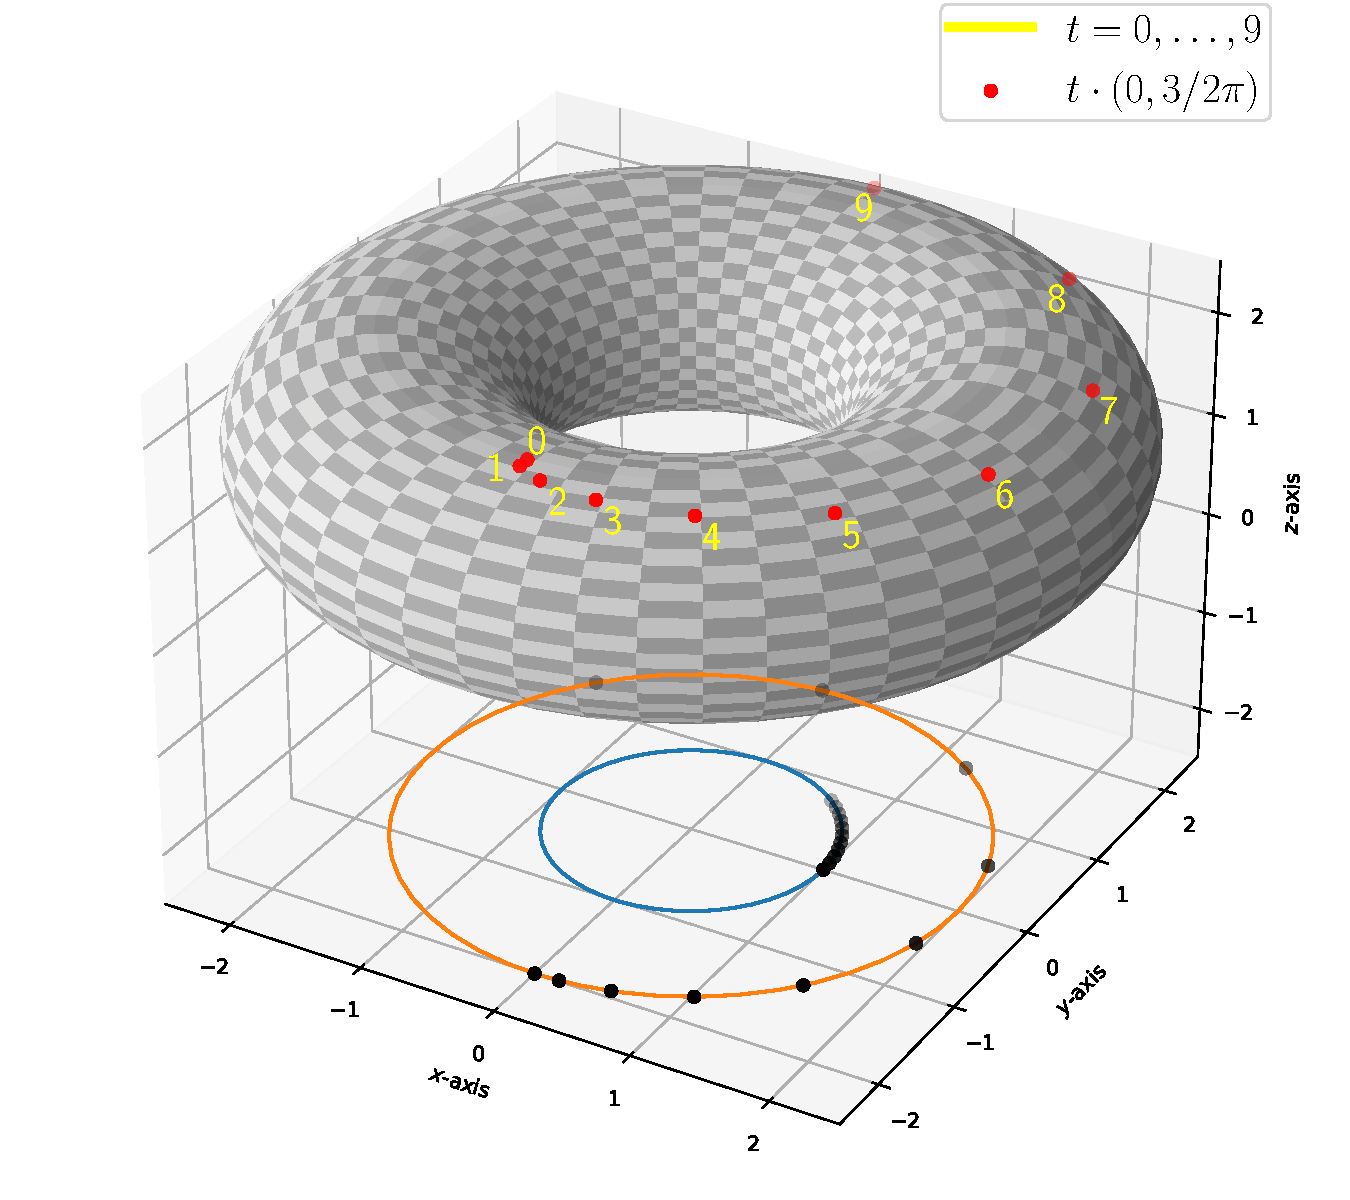
\includegraphics[width=8cm]{imgs/torusSkewRot.pdf}
    \end{column}
    \begin{column}{0.4\textwidth}
  \begin{example}[MEF of skew rotation]
Let $a \in \mathbb{T}$. Homeomorphism:
\begin{equation*}
  \begin{split}
    &\alpha: \mathbb{T}^2 \to \mathbb{T}^2,\\
  &\alpha (z,w) \coloneq (az,zw).
  \end{split}
  \end{equation*}
     TDS $(\mathbb{T}^2,\mathbb{Z})$, $\mathbb{Z}$-action:
     \begin{equation*}
     t \cdot (z,w) \coloneq \alpha^t (z,w).
     \end{equation*}
     \pause
  MEF is 
  \begin{equation*}
    \begin{split}
     &\pr_1 : (\mathbb{T}^2,\mathbb{Z}) \to (\mathbb{T},\mathbb{Z}), \\
    &\pr_1 (z,w) \coloneq z.
    \end{split}
  \end{equation*}
  $\mathbb{Z}$-action on $\mathbb{T}$:
  \begin{equation*}
   t\cdot  z \coloneq a^tz.
  \end{equation*}
\end{example}
       \end{column}
  \end{columns}
\end{frame}
\subsection{Relationship to measure preserving system concepts}
\begin{frame}{TDS with invariant measure as MPS}
Let $(X,T)$ a TDS, $T$ abelian, $\mu$ a $T$-invariant probability measure on $X$.
\begin{itemize}
  \item $(X,T,\mu)$ is a concrete measure preserving system (MPS)
  \item \emph{MPS Koopman operator}
\begin{equation*}
  \begin{split}
    &V : T \to L(L^2(X)),\\
    & (V(t) f)(x) \coloneq f (t x). 
  \end{split}
\end{equation*}
\item
  $(X,T,\mu)$ has \emph{MPS discrete spectrum} if and only if
  \begin{equation*}
    L^2(X) = \clin \bigcup_{\chi \in T^*} \ker (V - \chi).
  \end{equation*}
\end{itemize}
\pause
\begin{proposition}
  If $(X,T)$ has TDS discrete spectrum, then $(X,T,\mu)$ has MPS discrete spectrum.
  \end{proposition}
  The converse is false.
\end{frame}
\begin{frame}[fragile]{MEF is subsystem of the Kronecker subsystem}
  Let $\pi : (X,T) \to (X_m,T)$ be the MEF of $(X,T)$.
  \begin{itemize}
    \item $(X_m,T, \nu)$ with $\nu(A)\coloneq  \mu(\pi^{-1}(A))$ is concrete MPS with discrete spectrum,
  \item $\mathcal{X}, \mathcal{X}_m$ the MPS associated to $(X,T,\mu), (X_m,T,\nu)$ and $\pi^* : \mathcal{X}_m \to \mathcal{X}$ the induced extension,
  \item Let $K: \mathcal{K} \to \mathcal{X}$ the Kronecker subsystem of $\mathcal{X}$,
  \item Kronecker subsystem maximality: $\exists$ extension $J: \mathcal{X}_m \to \mathcal{K}$:
\end{itemize}
  \begin{center}
    \begin{tikzcd}[sep=large]
      \mathcal{X}_m \arrow[d, "J"'] \arrow[r, "\pi^*"]  \arrow[dr, phantom, "\circlearrowleft", near start] 
      & \mathcal{X}  \\
      \mathcal{K}  \arrow[ur,"K"'] & \phantom{a} \\
    \end{tikzcd}
  \end{center}
  \end{frame}

